%!TEX root = ../main.tex

\chapter{Schlüsseltechnologie nachhaltige Energiespeichersysteme}
\label{sec:einleitung}

\begin{quote}\glqq The fourth human energy revolution has begun.\grqq~\cite{Zhan.2018}\end{quote} 

Diese These stellen \textcite{Zhan.2018} in ihrem Buch zu Anwendungen und Grundlagen der Redox-Flow-Batterie auf. Damit ist der Ersatz fossiler durch regenerative Energiequellen und die damit verbundene Dekarbonisierung gemeint. Eine nachhaltige Entwicklung und der Fortbestand der menschlichen Entwicklung sollen damit gewährleistet werden. Mit Blick auf die Historie der Energietechnologien ist sie als vierte Revolution betitelt. Einzuordnen nach der Nutzung von Feuer, der Nutzung von fossilen Energieträgern und schließlich der flächendeckenden Bereitstellung von elektrischer Energie \cite{Zhan.2018}.

\begin{figure}[H]
    \centering
    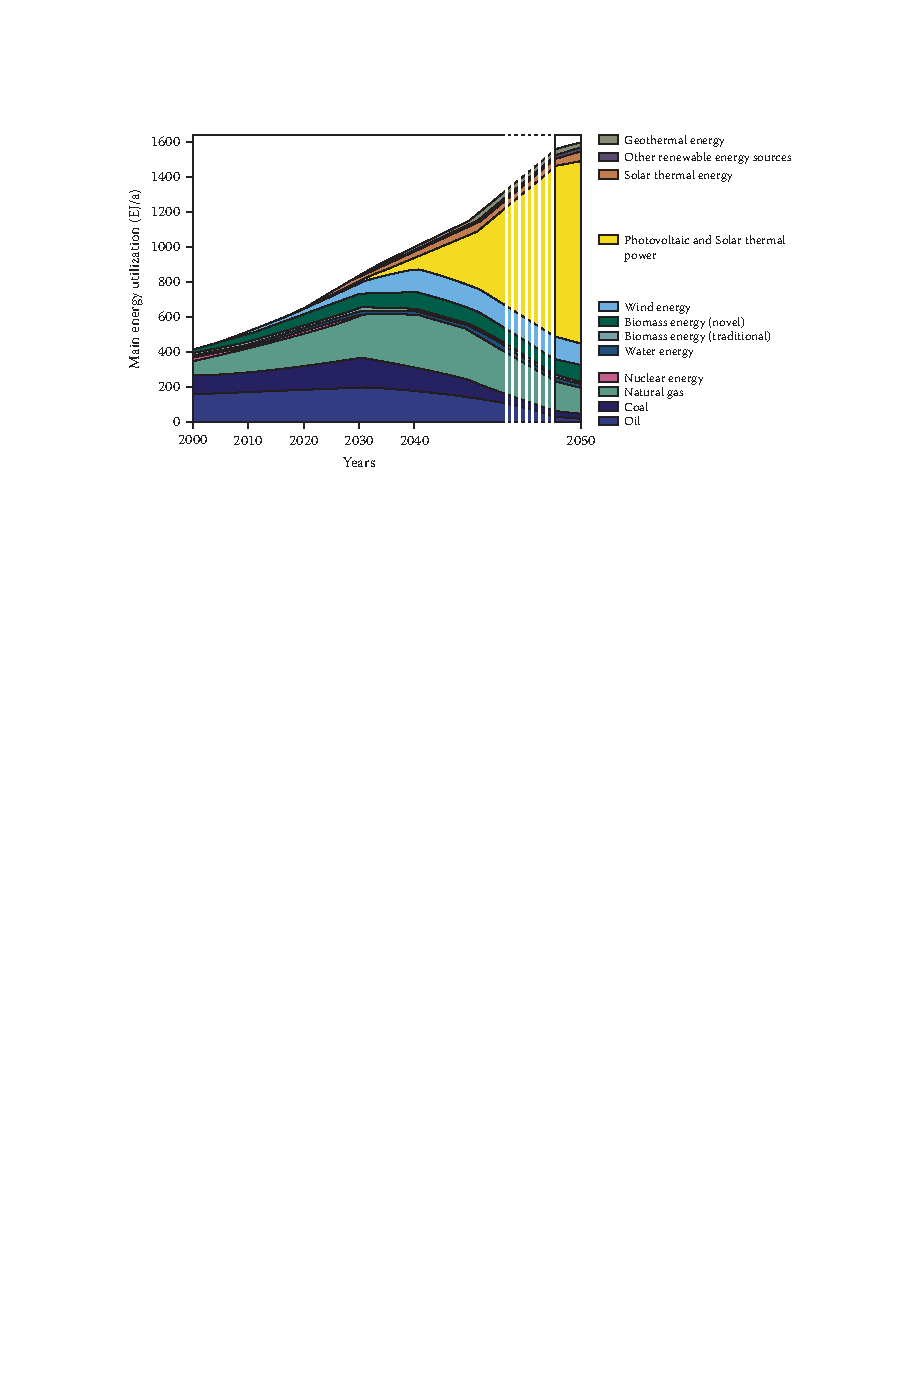
\includegraphics[width=\textwidth]{images/01kapitel/demand_primary_energy.pdf}
    \caption[Prognose des globalen Energiebedarfs]{Entwicklungsprognose des weltweiten Energiebedarfs mit absoluter Verteilung des Ursprunges aus primären Energiequellen; Stand 2010 \cite{Zhan.2018}}
    \label{fig:Demand_Energy}
\end{figure}

Die vierte Revolution des Energiesektors stellt Ingenieure vor Schwierigkeiten und Hürden. Ein weltweit wachsender absoluter Energiebedarf (siehe \autoref{fig:Demand_Energy}) setzt neben den zeitvariant verfügbaren regenerativen Energiequellen zusätzliche Ansprüche an die Entwicklungsperformance. Um dem entgegen zu wirken, entstanden einige Ansätze, z.B. \acp{ESS} zum Puffern von überschüssig produzierter Energie. Mit diesen Systemen sind auch weitere Szenarien, wie Smart Grids oder Microgrids zur lokalen Netzauskopplung und intelligenten Energieversorgung denkbar \cite{Zhan.2016, Esca.2018, Wess.2013, Turk.2013, Dhun.2020, Leop.2014, Ton.2012}.

Oft sind \acs{ESS} als Schlüsseltechnologie für den Wechsel in der Verwendung von primär fossilen zu regenerativen Energiequellen ausgewiesen \cite{Wess.2013, Zhan.2018, Ster.2016,Zapf.2017}. Durch die Erhöhung der Verfügbarkeit können regenerative Quellen, wie Wind- oder Solarenergie, zur Bewältigung der Grund- und Mittellast verwendet werden. Eine vielversprechende Speichertechnologie für stationäre Großspeicheranlagen ist neben der elektrochemischen Wasserstoffnutzung die \ac{RFB} \cite{Zhan.2018, Ster.2016}.

%%%%%%%%%%%%%%%%%%%%%%%%%%%%%%%%%%%%%%%%%%%%%%%%%%%%%%%%%%%%%%%%%%%%%%%%%%%%%
%%%%%%%%%%%%%%%%%%%%%%%%%%%%%%%%%%%%%%%%%%%%%%%%%%%%%%%%%%%%%%%%%%%%%%%%%%%%%
\section*{Motivation und Themenfindung}
\label{sec:themenfindung}
Bei einem Blick auf die Projektlandschaft bei Schaeffler existieren drei wesentliche Entwicklungsprojektarten, gegliedert nach Reifegrad des Produktes bzw. des Projektes. Der \ac{PEP} ist am nächsten an der Serie und hat zum Ziel fertige (Serien-) Produkte zu entwickeln, für welche bereits Kunden akquiriert worden sind. Das \ac{VEP} ist einen Reifegrad zuvor. Für Schaeffler unerforschte Technologien und Produkte werden entwickelt, um ein Vorserienprodukt zu erhalten. Dieses ist noch nicht auf große Stückzahlszenarien oder kundenspezifische Anforderungen optimiert. Am Anfang der Projektlandschaft steht das \ac{FIP}. Mit diesem werden in kurzer Zeit Innovationsideen über flexibel gestaltbare Demonstrator- bzw. Testprojekte analysiert und auf eine Übergabe in einen Geschäftsbereich (Business Unit) evaluiert. Neben des zunehmenden Produktreifegrades sind auf dieser Projektlandschaft die abnehmende Anzahl der Projekte zu nennen. \acp{FIP} bearbeiten eine größere Zahl an unterschiedlichen Projekten und Technologien im Vergleich zu den beiden seriennäheren Projektarten.

Genau an dieser Evaluation setzt vorliegende Bachelorarbeit an. Mehrere \acs{FIP}-Projekte mit dem Projektgegenstand einer \acs{RFB} sind auf einem bewertungswürdigen Stand. An diesem müssen sowohl die weiteren technischen Möglichkeiten abgeschätzt werden, um einem Serienprodukt gerecht werden zu können. Des Weiteren ist auch eine Sicht auf den Markt und die potenziellen Kunden des Produktes notwendig. So kann über die Kostenstruktur der Entwicklungen eine Einordnung am Markt erfolgen. Dieser gibt Aufschluss über die Verkaufswürdigkeit des Produktes, potenzielle Kunden und Business Cases. Diese wirtschaftlichen Dinge sind, neben der Technik, fortan wichtig bei einer Übergabe der zugehörigen Projekte an einen Geschäftsbereich. So ist das Ziel dieser Bachelorarbeit eine Antwort auf folgende Fragen:

\begin{quote}
    \glqq Welche Chancen und Perspektiven ermöglicht die Weiterentwicklung eines Redox-Flow-Batterie Stacks, im Sinne eines Transfers von einem \acf{FIP} zu einem (Vor-) Serienprojekt, aus technischer und ökonomischer Sichtweise?\\
    Welches Elektrodenkonzept stellt den besten technisch wirtschaftlichen Kompromiss als Aktivmaterialkomponente für eine Weiterentwicklung dar?\grqq
\end{quote}

%%%%%%%%%%%%%%%%%%%%%%%%%%%%%%%%%%%%%%%%%%%%%%%%%%%%%%%%%%%%%%%%%%%%%%%%%%%%%
%%%%%%%%%%%%%%%%%%%%%%%%%%%%%%%%%%%%%%%%%%%%%%%%%%%%%%%%%%%%%%%%%%%%%%%%%%%%%
\section*{Vorgehen und Aufbau}
Das Vorgehen, um Antworten auf vorangegangene Fragen zu finden, entwickelt sich aus verschiedenen relevanten Teilbereichen und den beschriebenen Überlegungen im Hintergrund. Diverse Methoden aus dem Ingenieurwesen, aber auch aus der wirtschaftswissenschaftlichen Arbeitsweise finden Anwendung. Die Aufarbeitung einer Marktanalyse in Kombination mit einer Patentrecherche legt sowohl einen Stand der Technik als auch das Verhalten am Batteriemarkt dar. So kann das eigene System in Relation gesetzt werden. Eine transparentes Kostenbewusstsein ermöglicht die Bewertung des ökonomischen Parts. Aufbauend kategorisiert eine technisch-wirtschaftliche Lösungsbewertung die verschiedenen Elektrodenkonzepte. Durch die Diskussion aller Teilbereiche kann ein Aussprechen von Empfehlungen erfolgen. So ergibt sich folgender Aufbau der vorliegenden Arbeit:

\begin{onehalfspace}
    \begin{itemize}
        \item \textbf{Kapitel \ref{sec:grundlagen}}\\ordnet die Technologie ein und legt die technischen Grundlagen von \acsp{RFB} und in der Arbeit relevanter Technik dar.
        \item \textbf{Kapitel \ref{sec:stand-technik}}\\nutzt Recherchemethoden, um einen Überblick über den Markt und aktuelle Patente zu geben.
        \item \textbf{Kapitel \ref{sec:stackanalyse}}\\beschreibt den technischen Aufbau des projektierten Stacks und dessen Auslegungsprozess.
        \item \textbf{Kapitel \ref{sec:kostenstruktur}}\\behandelt die Ableitung der Kostenstruktur des Stacks.
        \item \textbf{Kapitel \ref{sec:t-w-betrachtung}}\\führt eine Technisch-Wirtschaftliche Analyse verschiedener Elektrodenkonzepte durch.
        \item \textbf{Kapitel \ref{sec:diskussion}}\\diskutiert Optimierungspotentiale auf Basis der vorangegangenen Kapitel.
        \item \textbf{Kapitel \ref{sec:fazit}}\\fasst zusammen und reflektiert die Methoden kritisch. Ein Ausblick der Technologie und weiterer Ansatzpunkte wird gegeben.
    \end{itemize}
\end{onehalfspace}

